% !TEX program = lualatex
% Compile from 2026/week13; figures are generated by make_figures.py.
\documentclass[12pt,aspectratio=43]{beamer}
% Shared Beamer design. Load after \documentclass using \input.
% Engine: LuaLaTeX. Fonts: UD Digi Kyokasho N (regular/bold), Arial.
\usepackage{luatexja-fontspec}
\setmainjfont[BoldFont={UD Digi Kyokasho N Bold}]{UD Digi Kyokasho N}
\setsansjfont[BoldFont={UD Digi Kyokasho N Bold}]{UD Digi Kyokasho N}
\setmonojfont[BoldFont={UD Digi Kyokasho N Bold}]{UD Digi Kyokasho N}
% Liberation Sans keeps the layout usable on systems without Arial.
\IfFontExistsTF{Arial}{
  \setmainfont{Arial}
  \setsansfont{Arial}
  \setmonofont{Arial}
}{
  \setmainfont{Liberation Sans}
  \setsansfont{Liberation Sans}
  \setmonofont{Liberation Sans}
}
\renewcommand{\kanjifamilydefault}{\gtdefault}

% Typeset mathematics with a dedicated TeX math font, independent of Arial.
\usefonttheme{professionalfonts}
\usepackage[mathrm=sym]{unicode-math}
\setmathfont{Latin Modern Math}
\setoperatorfont{\symup}

\definecolor{courseblue}{HTML}{4472C4}
\definecolor{ruleblue}{HTML}{8FAADC}
\setbeamercolor{normal text}{fg=black,bg=white}
\setbeamercolor{structure}{fg=courseblue}
\setbeamercolor{frametitle}{fg=black,bg=white}
\setbeamercolor{title banner}{fg=white,bg=courseblue}
\setbeamerfont{frametitle}{size=\fontsize{18}{22}\selectfont,series=\mdseries}
\setbeamerfont{quote}{shape=\upshape}
\setbeamersize{text margin left=9mm,text margin right=9mm}
\setbeamertemplate{navigation symbols}{}
\setbeamercolor{page number}{fg=gray,bg=white}
\setbeamertemplate{footline}{%
  \begin{beamercolorbox}[wd=\paperwidth,ht=2.5mm,dp=1.5mm]{page number}
    \hfill{\fontsize{8}{9}\selectfont
      \ifnum\value{framenumber}>0
        \insertframenumber\,/\,\inserttotalframenumber
      \fi}\hspace*{3mm}
  \end{beamercolorbox}}
\setbeamertemplate{headline}{%
  \hfill\textcolor{gray}{\fontsize{6}{7}\selectfont
    \hypersetup{linkcolor=gray}% Keep Beamer's title links in the header color.
    \ifnum\value{framenumber}=0 \insertshortdate\enspace\fi
    \insertshorttitle\space\insertshortsubtitle}\hspace{2mm}\vspace{1.5mm}}
\setbeamertemplate{frametitle}{%
  \vspace{2mm}\centering\insertframetitle\par
  \vspace{-1mm}{\color{ruleblue}\rule{.44\paperwidth}{.5pt}}\par
  \vspace{2mm}}
\setbeamercolor{itemize item}{fg=courseblue}
\setbeamercolor{itemize subitem}{fg=black}
\setbeamercolor{itemize subsubitem}{fg=black}
\setbeamertemplate{itemize item}{\textbullet}
\setbeamertemplate{itemize subitem}{\textnormal{-}}
\setbeamertemplate{itemize subsubitem}{\textnormal{-}}
\setlength{\parskip}{.45em}
\hypersetup{colorlinks=true,urlcolor=courseblue}

% Use \titlepage inside a [t,noframenumbering] frame. The background extends
% 1 mm past both page edges to avoid hairline gaps in PDF viewers.
\setbeamertemplate{title page}{%
  \vspace{2mm}
  \begin{beamercolorbox}[wd=\paperwidth,ht=43mm,dp=13mm,colsep*=1mm,center]{title banner}
    {\fontsize{32}{40}\selectfont\inserttitle\par}
    \vspace{2mm}
    {\fontsize{20}{24}\selectfont\insertsubtitle\par}
  \end{beamercolorbox}
  \vspace{10mm}
  \hfill\insertauthor
}

\graphicspath{{figures/}}
\usepackage{listings}
\usepackage{upquote}
\IfFontExistsTF{Consolas}{\newfontfamily\codefont{Consolas}}{\newfontfamily\codefont{Liberation Mono}}
\definecolor{codevalue}{HTML}{7A3E9D}
\definecolor{codebuiltin}{HTML}{006DB0}
\definecolor{codestring}{HTML}{267348}
\newcommand{\code}[1]{{\codefont #1}}
\lstdefinestyle{python}{
  language=Python,
  basicstyle=\codefont\fontsize{12}{14}\selectfont,
  keywordstyle=\color{codebuiltin},
  stringstyle=\color{codestring},
  showstringspaces=false,
  columns=fullflexible,
  keepspaces=true,
  upquote=true,
  tabsize=4,
  breaklines=false,
  backgroundcolor=\color{black!4},
  frame=single,framerule=0pt,framesep=1.7mm,
  xleftmargin=1.7mm,xrightmargin=1.7mm,
  aboveskip=1mm,belowskip=0.5mm,
  literate=*{0}{{{\color{codevalue}0}}}1
    {1}{{{\color{codevalue}1}}}1 {2}{{{\color{codevalue}2}}}1
    {3}{{{\color{codevalue}3}}}1 {4}{{{\color{codevalue}4}}}1
    {5}{{{\color{codevalue}5}}}1 {6}{{{\color{codevalue}6}}}1
    {7}{{{\color{codevalue}7}}}1 {8}{{{\color{codevalue}8}}}1
    {9}{{{\color{codevalue}9}}}1
}
\lstset{style=python}
\setbeamercolor{lesson note}{fg=black,bg=courseblue!9}
\newenvironment{lessonbox}
  {\begin{beamercolorbox}[wd=\linewidth,sep=1.5mm]{lesson note}}
  {\end{beamercolorbox}\par}

\title{計算物理学B}
\subtitle{第十三回：偏微分方程式2}
\author{野垣 康介、藤本 悠輝}
\date{2027/1/26}
\hypersetup{pdftitle={計算物理学B 第十三回：偏微分方程式2},pdfauthor={野垣 康介、藤本 悠輝}}

\begin{document}

\begin{frame}[t,noframenumbering]
  \titlepage
\end{frame}

\begin{frame}{講義予定}
  \setlength{\parskip}{0pt}
  2026年度 第2学期（火曜3限）
  \par\vspace{2mm}
  \begingroup\centering
    \renewcommand{\arraystretch}{1.05}
    \begin{tabular}{@{}l@{\hspace{2mm}}l@{\hspace{4mm}}l@{\hspace{2mm}}l@{}}
      10/6 & 四則演算 & 12/8 & モンテカルロ1 \\
      10/27 & 制御文（for, if） & 12/15 & モンテカルロ2 \\
      11/6（金） & 関数 & 12/22 & 微分方程式1 \\
      11/10 & 配列（NumPy） & 1/12 & 微分方程式2 \\
      11/17 & 可視化（matplotlib） & 1/19 & 偏微分方程式1 \\
      11/24 & 数値微分 & 1/26 & \textcolor{courseblue}{\textbf{偏微分方程式2}} \\
      12/1 & 数値積分 & 2/2 & 根の探索 \\
      \multicolumn{2}{c}{\small 〜中間レポート〜} &
      \multicolumn{2}{c}{\small 〜期末レポート〜}
    \end{tabular}\par
  \endgroup
  \vspace{2mm}
  {\small \textcolor{courseblue}{10/20は出張で休講。} 11/6（金）は火曜授業の振替。\par}
\end{frame}

\begin{frame}{授業で使うリンク}
  \begin{itemize}
    \setlength{\itemsep}{3mm}
    \item Google Colab：{\small\url{https://colab.research.google.com/?hl=ja}}
    \item 講義資料（GitHub）：{\small\url{https://github.com/nogaki/Computational_Physics_B}}
    \item ノートブック案内：\code{2026/week13/week13.ipynb}
    \item 波動方程式：\code{2026/week13/Wave.ipynb}
    \item Schrödinger方程式：\code{2026/week13/Schrodinger.ipynb}
  \end{itemize}
\end{frame}

\begin{frame}[t]{Colabでノートブックを使う}
  \begin{enumerate}
    \setlength{\itemsep}{3mm}
    \item \code{week13.ipynb}を開き、二つのNotebookの実行順を確認する。
    \item \code{Wave.ipynb}、続いて\code{Schrodinger.ipynb}を開く。
    \item 各Notebookを上から実行する。
  \end{enumerate}
  \vspace{3mm}
  \begin{lessonbox}
    \textbf{各Notebookで「ドライブにコピーを保存」}\par
    \small GitHub上のNotebookを開いただけではDriveに保存されない。
  \end{lessonbox}
  \vfill
  {\footnotesize いずれも同じ週のフォルダに保存されている。}
\end{frame}

\begin{frame}[t]{今回の内容}
  \begin{itemize}
    \setlength{\itemsep}{3mm}
    \item 波動方程式：FTCS法、陰解法、Crank--Nicolson法
    \item 数値安定性と離散エネルギー
    \item 時間依存Schrödinger方程式
    \item ガウス波束の障壁散乱と確率保存
  \end{itemize}
  \vfill
  \begin{lessonbox}
    \code{Wave.ipynb}は前回の波動方程式の実習を完成させるNotebook。
  \end{lessonbox}
\end{frame}

\begin{frame}[t]{1次元の波動方程式}
  \[
    \frac{\partial^2\phi}{\partial t^2}
    =v^2\frac{\partial^2\phi}{\partial x^2}.
  \]
  \begin{itemize}
    \item 初期変位\(\phi(0,x)\)と初期速度\(\partial_t\phi(0,x)\)を指定する。
    \item Dirichlet条件：端の変位を指定する。固定端は\(\phi=0\)。
    \item Neumann条件：端の傾きを指定する。自由端は\(\partial_x\phi=0\)。
  \end{itemize}
  \small 固定端は変位の節、自由端は変位の腹に対応する。
\end{frame}

\begin{frame}[t]{2階の時間微分を1階の連立系にする}
  \(\psi=\partial_t\phi\)とおけば
  \[
    \partial_t\phi=\psi,\qquad
    \partial_t\psi=v^2\partial_x^2\phi.
  \]
  格子幅を\(a=\Delta x\)、時間刻みを\(h=\Delta t\)とする。
  \[
    L\phi_k=\phi_{k+1}-2\phi_k+\phi_{k-1},\qquad
    r=\frac{hv^2}{a^2}.
  \]
  \begin{itemize}
    \item 端点を固定し、内部点\(k=1,\ldots,N-1\)を更新する。
    \item \(r\)は差分式の係数。波速と格子・時間刻みに依存する。
  \end{itemize}
\end{frame}

\begin{frame}[t]{FTCS法：前進Euler更新}
  \[
    \phi^{n+1}=\phi^n+h\psi^n,\qquad
    \psi^{n+1}=\psi^n+rL\phi^n.
  \]
  空間差分の固有モードは調和振動子になる。前進Euler更新の増幅率は
  \[
    |G|=\sqrt{1+(h\Omega)^2}>1\quad(\Omega\ne0).
  \]
  \begin{itemize}
    \item この1階連立系にFTCS法を使うと、時間刻みを小さくしても振幅が増える。
    \item ここで扱う不安定性は前進Euler更新についての結論。他の差分式には別の安定条件がある。
  \end{itemize}
\end{frame}

\begin{frame}[t]{陰解法：安定だが振動は減衰する}
  \[
    \phi^{n+1}=\phi^n+h\psi^{n+1},\qquad
    \psi^{n+1}=\psi^n+rL\phi^{n+1}.
  \]
  \(\phi^{n+1}\)を消去すると
  \[
    (I-rhL)\psi^{n+1}=\psi^n+rL\phi^n.
  \]
  \begin{itemize}
    \item 内部点ごとに三重対角方程式を解く。
    \item 時間更新は安定だが、調和振動子の振幅を小さくする。
    \item 大きな刻み幅ほど数値減衰が強くなる。
  \end{itemize}
\end{frame}

\begin{frame}[t]{Crank--Nicolson法}
  前時刻と次時刻の右辺を平均する。
  \[
    \phi^{n+1}=\phi^n+\frac h2(\psi^{n+1}+\psi^n),
  \]
  \[
    \psi^{n+1}=\psi^n+\frac r2L(\phi^{n+1}+\phi^n).
  \]
  \begin{itemize}
    \item 陰解法と同じく三重対角方程式を解く。
    \item 調和振動子の振幅と離散エネルギーを保つ。
    \item 波動方程式の時間更新に適した選択肢となる。
  \end{itemize}
\end{frame}

\begin{frame}[t]{Crank--Nicolson法の三重対角方程式}
  \(\psi^{n+1}\)について整理すると
  \[
    (4I-rhL)\psi^{n+1}
    =(4I+rhL)\psi^n+4rL\phi^n.
  \]
  内部点では
  \[
    -rh\psi^{n+1}_{k-1}+(4+2rh)\psi^{n+1}_k-rh\psi^{n+1}_{k+1}
  \]
  \[
    =4\psi^n_k+4rL\phi^n_k+rhL\psi^n_k.
  \]
  この方程式を解いた後、\(\phi^{n+1}\)を時間平均の式で求める。
\end{frame}

\begin{frame}[t]{方法ごとの離散エネルギー}
  固定端の波動方程式の離散エネルギーを
  \[
    E=\frac{a}{2}\sum_k\psi_k^2
    +\frac{v^2}{2a}\sum_k(\phi_{k+1}-\phi_k)^2
  \]
  とする。
  \begin{itemize}
    \item FTCS：時間刻みにかかわらず増幅する。
    \item 陰解法：安定だがエネルギーが減る。
    \item Crank--Nicolson：この線形系の離散エネルギーを保つ。
  \end{itemize}
\end{frame}

\begin{frame}[t]{同じ初期モードで比較}
  \centering
  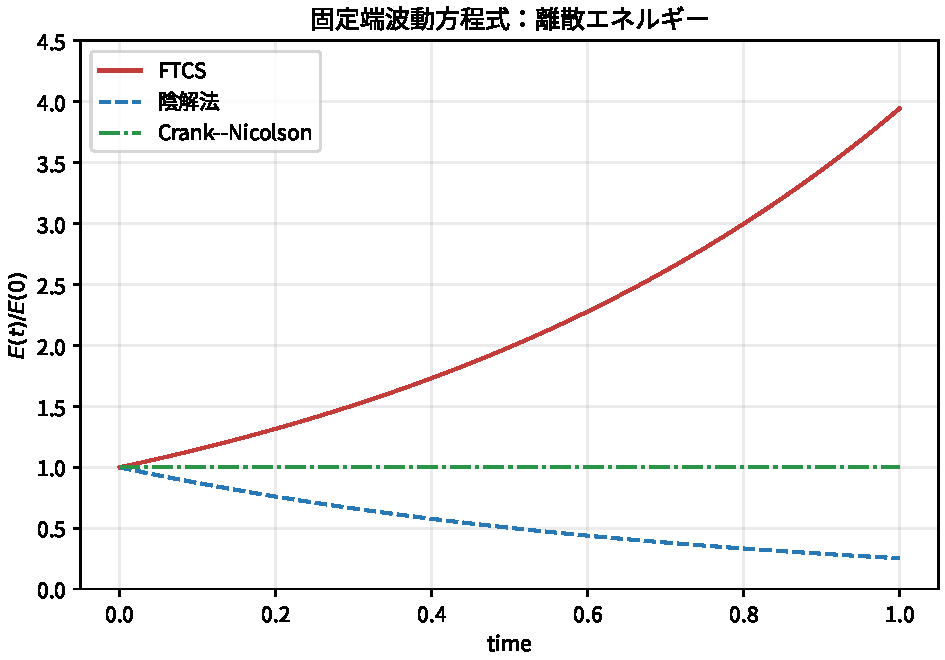
\includegraphics[width=.76\linewidth,height=45mm,keepaspectratio]{wave_energy.pdf}
  \par\vspace{2mm}
  \small \(N=100\)、モード40、\(v=0.1\)、\(h=0.01\)、\(t=1\)。初期速度は0。
  赤実線：FTCS、青破線：陰解法、緑一点鎖線：Crank--Nicolson。
\end{frame}

\begin{frame}[t]{時間依存Schrödinger方程式}
  \[
    i\hbar\frac{\partial\psi}{\partial t}
    =\left[-\frac{\hbar^2}{2m}\frac{\partial^2}{\partial x^2}+V(x)\right]\psi.
  \]
  以下では原子単位系を使う。
  \begin{itemize}
    \item \(\hbar=m_e=e=a_0=E_h=1\)。
    \item 位置はBohr半径\(a_0\)、エネルギーはHartree\(E_h\)。
    \item 時間は\(\hbar/E_h\)（約\(2.42\times10^{-17}\)秒）。
  \end{itemize}
  \small 確率密度は\(|\psi(x,t)|^2\)。
\end{frame}

\begin{frame}[t]{空間差分とHamiltonian行列}
  内部格子点では運動エネルギーを三重対角行列にする。
  \[
    T_{jj}=\frac{1}{a^2},\qquad
    T_{j,j\pm1}=-\frac{1}{2a^2}.
  \]
  \begin{itemize}
    \item Hamiltonianは\(H=T+\operatorname{diag}(V)\)。
    \item 端点の\(\psi=0\)を固定し、内部点だけを時間発展させる。
    \item 時間に依存しない実ポテンシャルなら\(H\)はHermite行列。
  \end{itemize}
\end{frame}

\begin{frame}[t]{時間発展：Crank--Nicolson法}
  \[
    \left(I+i\frac{h}{2}H\right)\Psi^{n+1}
    =\left(I-i\frac{h}{2}H\right)\Psi^n.
  \]
  \begin{itemize}
    \item 左辺は毎時刻同じ行列なので、LU分解を再利用できる。
    \item Hermiteな\(H\)に対して更新はユニタリ。
    \item 離散ノルム\(a\sum_j|\psi_j|^2\)は保存される。
  \end{itemize}
  \begin{lessonbox}
    ノルム保存は実装の確認指標。位置格子を細かくした結果も比べる。
  \end{lessonbox}
\end{frame}

\begin{frame}[t]{ガウス波束と矩形障壁}
  初期波束を
  \[
    \psi(x,0)=\frac{1}{(\pi\sigma^2)^{1/4}}
    e^{-(x-x_0)^2/(2\sigma^2)}e^{ik_0(x-x_0)}
  \]
  とする。
  \begin{itemize}
    \item \(x_0=-10\,a_0\)、\(\sigma=1.8\,a_0\)、\(k_0=10\,a_0^{-1}\)。
    \item 波数\(k_0\)に対応する運動エネルギーの中心値は\(k_0^2/2=50\,E_h\)。
    \item 高さ\(36.2\,E_h\)、幅\(0.5\,a_0\)の障壁を原点に置く。
  \end{itemize}
  \small 平均エネルギーより低い障壁でも、散乱による反射が起こる。
\end{frame}

\begin{frame}[t]{波束の散乱：計算結果}
  \centering
  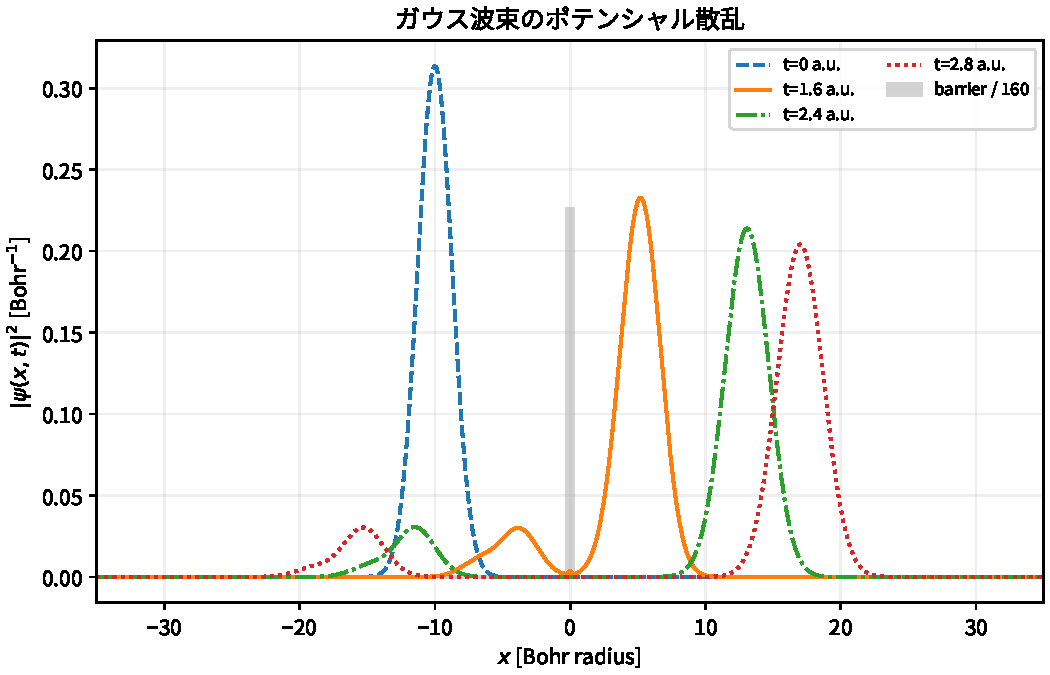
\includegraphics[width=.88\linewidth,height=48mm,keepaspectratio]{wave_packet_scattering.pdf}
  \par\vspace{1mm}
  \small \(x\in[-40,40]\,a_0\)、3200区間、\(\Delta t=0.004\)、最終時刻2.8 au。
  灰色は高さを160で割った障壁、線種は\(t=0,1.6,2.4,2.8\) au。
\end{frame}

\begin{frame}[t]{ノルム・反射確率・透過確率}
  散乱後に左右の領域で確率密度を積分する。
  \[
    P_R=\int_{x<0}|\psi(x,t)|^2\,dx,\qquad
    P_T=\int_{x>0}|\psi(x,t)|^2\,dx.
  \]
  \begin{itemize}
    \item 3200区間では\(t=2.8\) auで\(P_R\simeq0.1331\)、\(P_T\simeq0.8669\)。
    \item 区間数を6400にすると\(P_R\simeq0.1392\)、\(P_T\simeq0.8608\)。
    \item \(\int|\psi|^2dx\)の時間変化は\(10^{-10}\)以下。
    \item これらは格子に依存する離散値で、連続系の収束値ではない。
  \end{itemize}
\end{frame}

\begin{frame}[t]{有限領域と境界反射}
  \begin{itemize}
    \setlength{\itemsep}{3mm}
    \item Dirichlet境界\(\psi=0\)は反射壁として働く。
    \item 端で反射した波が戻る前に、散乱領域の確率を測る。
    \item 計算時間を長くする場合は、箱を広げて結果を比べる。
    \item 遅い波束ほど境界に届くまでの時間が長い。
  \end{itemize}
  \vfill
  \begin{lessonbox}
    確率保存を満たしていても、箱の端から戻った波が混ざることがある。
  \end{lessonbox}
\end{frame}

\begin{frame}[t]{実習：障壁を変えて散乱を調べる}
  \begin{itemize}
    \item \code{Schrodinger.ipynb}で障壁の高さ・幅・形状を変える。
    \item 反射・透過確率がどう変わるかを比較する。
    \item 計算時間を延ばしたとき、境界反射が結果に混ざらないか調べる。
    \item Crank--Nicolson法の離散ノルム保存も確認する。
  \end{itemize}
  \vfill
  \begin{lessonbox}
    Notebook末尾の実習セルは空欄。条件を変えて自分で計算する。
  \end{lessonbox}
\end{frame}

\begin{frame}[t]{まとめと参考}
  \begin{itemize}
    \item 波動方程式の時間更新法は、エネルギーの増幅・減衰・保存が異なる。
    \item Schrödinger方程式のCrank--Nicolson法は離散確率を保つ。
    \item 境界条件と観察時間を選び、反射の影響を確認する。
  \end{itemize}
  \vfill
  {\footnotesize
    野本拓也・是常隆・有田亮太郎『実践計算物理学』共立出版。\\
    Z. Q. Jin, \emph{Numerical solution of the time-dependent Schrödinger equation}.\\
    \url{http://staff.ustc.edu.cn/~zqj/posts/Numerical_TDSE/}\\
    \url{https://github.com/vlvovch/PHYS6350-ComputationalPhysics}}
\end{frame}

\end{document}
